\documentclass[10pt,twocolumn,letterpaper]{article}

\usepackage{iccp}
\usepackage{times}
\usepackage{amsmath}
\usepackage{amssymb}
\usepackage{url}
\usepackage{graphicx}
\DeclareMathOperator*{\argmin}{\arg\!\min}
% for rapid builds, with bounding boxes instead of images add the [draft] option to graphicx
% \usepackage[draft]{graphicx}

\iccpfinalcopy % *** Uncomment this line for the final submission

\def\iccpPaperID{****} % *** Enter the ICCP Paper ID here
\def\httilde{\mbox{\tt\raisebox{-.5ex}{\symbol{126}}}}

% Pages are numbered in submission mode, and unnumbered in camera-ready
\ificcpfinal\pagestyle{empty}\fi
\begin{document}

%%%%%%%%% TITLE
\title{Comparison of Sparsity in Different Basis for Lightfields}

\author{Philip K. Lee\\
Stanford University\\
Electrical Engineering Department\\
{\tt\small pkl.lee@stanford.edu}
\and
Anqi R. Ji\\
Stanford University\\
Electrical Engineering Department\\
{\small\url{anqi@stanford.edu}}
}

\maketitle
\thispagestyle{empty}

%%%%%%%%% ABSTRACT
\begin{abstract}
Lightfield camera images provide not only spatial information but also angular information. This allows us to refocus, capture depth map and create all-in-focus images which are impossible in the post-processing of conventional camera images. There are three main types of lightfield camera: microlens array lightfield camera, sequential capturing lightfield camera and multi-camera array. Due to its compact size and easy calibration, lightfield cameras using microlens arrays are the only method among these three that have been commercialized. However, an inherent trade-off between the spatial and angular resolution resulting in an overall loss of resolution exists in this type of lightfield camera. In this paper, we apply compressive sensing in order to overcome this resolution limitation by assuming sparsity in some basis. We simulate multiple captures using random attenuation masks placed in front of the aperture, and reconstruct the image using basis pursuit in the Fourier, discrete cosine, and Haar wavelets basis, and compare it to reconstructions using a sparse gradient prior. We evaluate the performance of these methods by comparing their SNRs at different compression factors. 
\end{abstract}

\section{Introduction}

Different methods of capturing the 4D light field exist, which balance a tradeoff between spatial and angular resolution, and require additional hardware and capture times. These methods include a microlens array mounted in front of the camera sensor \cite{NgLF}, which comes at the cost of spatial resolution, and camera arrays \cite{LFArray} or cameras mounted on a mechanical gantry \cite{LFRendering}. Sparse reconstruction of the light field is desirable as it helps to alleviate some of these tradeoffs. Priors that exploit the sparsity of the light field in some dimension allow the entire light field to be reconstructed from a limited number of samples. For example, the light field can be considered to be sparse in the angular domain due to the light field being the same scene acquired from slightly different perspective. 

Multiple methods have been applied to reconstruct the light field from a sparse set of samples. 

In \cite{DimGapLFPrior}, a Lambertian scene is assumed and a 3D Gaussian prior is applied to the scene. This prior comes from the observation that the 4D Fourier transform of the 4D ray space contains a 3D subset of entries whose energy is significantly higher than zero. Under this prior, the light field can be recovered using spatial deconvolutions with a depth invariant Point Spread Function. Though this method is easy to compute, it creates artifacts in non-Lambertian scenes.

A second approach applied in \cite{LFDict} recovers the light field using a randomly coded attenuation mask and dictionaries derived from training data acquired from other light field images. The dictionaries are then applied to solve the ill-posed problem of recovering the entire light field from a random linear combination of light field samples provided by the coded mask.

Compressive sensing \cite{IntroCS}\cite{CompressiveSensingMega} is another approach to reconstruction of the light field using sparse samples. The approach is similar to that of the single pixel camera \cite{SinglePixelCamera}, which samples random projections of the image and reconstructs the original image from the samples. By applying a randomly-coded aperture mask to the lens, the authors of \cite{SparsityInCFD} were able to reconstruct the light field with a superior angular resolution and SNR compared to sequentially opening and blocking small regions of the aperture. The light field is recovered using a Bayesian reconstruction model with Total Variation and Gaussian priors. A Majorize-Minimization optimization was used to recover the light field.

In order to achieve the best reconstruction using compressive sensing, it is desirable to perform the reconstruction in the basis in which the original signal is most sparse, as a higher percentage of the signal's energy will be concentrated in fewer coefficients of the sparse basis \cite{CompressiveSensingMega}. Therefore it is advantageous to determine in what basis the angular lightfield is most sparse. This was explored in part in \cite{mainP1}, but only the basis that yielded the best reconstruction for each compression was shown. The goal of our work is to experimentally determine the basis in which lightfields are most sparse by performing sparse reconstructions of the lightfield for different compression factors. We use images captured from a Lytro Illum camera available from the Stanford Lytro Light Field Archive \footnote{Available: \url{lightfields.stanford.edu}} to simulate measurements and determine the reconstruction error for different basis.

\section{Background}

In the background, we present the basic mathematics for compressed sensing and recovery using the total variance prior.

\subsection{Compressed Sensing}

In this section we present the formulation of the compressed sensing framework \cite{CSPaper} for the general case and for lightfields. A signal $x \in \mathbb{R}^N$ which is $K$-sparse in some basis $\Phi \in \mathbb{R}^{N\times N}$, i.e.,

\[ x = \Phi \theta, \quad ||\theta||_0 = K, \quad K \ll N\]

can be recovered using a smaller vector $y \in \mathbb{R}^M, M < K < N$, where $y$ is a vector consisting of linear combinations of $x$. In matrix notation, $y$ can be expressed as 

\[ y = \Psi x, \quad \Psi \in \mathbb{R}^{M \times N}\]

$\Psi$ is known as the sensing matrix. There are many ways to generate $\Psi$ that would allow for sparse recovery using a limited number of measurements. One such method is to use a $\Psi$ whose elements are drawn from a Gaussian or Bernoulli distribution, but this choice is determined by the physical limitations of the problem \cite{Rauhut11}. The vector $x$ can be recovered as $\hat{x}$ if $M$ is large enough ($M \sim K\log(N/K)$) by finding the optimum solution for 

\[ \hat{\theta} = \argmin_\theta ||\theta||_0 \quad s.t. \quad \Psi\Phi\theta = y\]

and recovering $\hat{x}$ using

\[ \hat{x} = \Phi \hat{\theta}\]

Intuitively, this optimization seeks to concentrate the energy of the reconstructed signal in as few coefficients as possible in the sparse basis, while also ensuring that applying the sensing matrix to the reconstructed signal is close to the measurements. However, $l_0$ optimization is NP-hard, so instead we resort to the $l_1$ norm which approximates the $l_0$ norm

\[ \hat{\theta} = \argmin_\theta ||\theta||_1 \quad s.t. \quad \Psi\Phi\theta = y\]

This problem is known as Basis Pursuit (BP) \cite{BasisPursuit1}. For the general case with added noise in the measurements, the problem becomes

\[ \hat{\theta} = \argmin_\theta ||\theta||_1 \quad s.t. \quad ||\Psi\Phi\theta - y||_2 < \sigma\]


where $\sigma$ is a bound for the noise in the measurements. This is the Basis Pursuit Denoise (BPDN) problem. In our work, we only consider Basis Pursuit.

\subsection{Compressed Sensing for Lightfields}

In the background, we considered the reconstruction of signals in 1 dimension. However, a lightfield exists in 4 dimensions: the spatial dimensions $x, y$ and the angular dimensions $u, v$. In this section, we will recast the problem in terms of the dimensions for a 4D lightfield. Note that the dimensions for the matrix multiplications may not align, but this section is included to clarify the reconstruction for 4D lightfields.

Consider a lightfield $L \in \mathbb{R}^{w \times h \times n \times n}$, where $w$ and $h$ are respectively the width and height of each angular image. For simplicity, we assume that the number of angular lightfield views $n$ is equal in each dimension. We wish to recover $L$ using only linear combinations of $L$.

Our sensing matrix $\Psi$ operates on the angular images, therefore $\Psi$ is of size $\mathbb{R}^{M \times n \times n}$ where $M$ is the number of measurements. Our measured data is therefore

\[Y = \Psi L, \quad Y \in \mathbb{R}^{w \times h \times M}\]

The orthogonal basis $\Phi$ operates in the angular domain, so $\Phi \in \mathbb{R}^{n \times n}$. The BP problem becomes

\[ \hat{\theta} = \argmin_\theta ||\theta||_1 \quad s.t. \quad \Psi\Phi\theta = Y\]
\[ \hat{\theta}, \theta \in \mathbb{R}^{w \times h \times n \times n}\]

and the lightfield is recovered using

\[ \hat{L} = \Phi \hat{\theta}\]

To solve the BP problem, it is convenient to let the matrix $A = \Psi\Phi$. We can now define the adjoint operator as $A' = \Phi'\Psi'$ where the $'$ denotes the transpose. Since $\Phi$ is orthonormal, $\Phi'\Phi = I$, so $\Phi'$ is the inverse of the basis operator. 

The above formulation can also be recast using the framework presented in \cite{GordonArticle2}, but this is not presented in this work.

\subsection{Total Variation Prior}

Unlike compressed sensing which assumes sparsity in some orthogonal basis, Total Variation (TV) assumes sparsity in the gradients of the image. This is achieved by minimizing the following cost function

\[ \hat{x} = \argmin_x ||Ax - b||^2_2 + \lambda ||D x||_1 \]

Where $D$ is the gradient operator and $\lambda$ is a parameter that can be chosen. A larger choice of $\lambda$ will reduce the amount of edges in the image. $A$ is similar to the sensing matrix presented above and constitutes the masks used to generate the measurements $b$.

\section{Methods}


24 images were chosen at random from the Stanford Lytro Light Field Archive \footnote{Available: \url{lightfields.stanford.edu}}. Images captured using the Lytro Illum camera have a raw resolution of $7574 \times 5264$ pixels, and has $14 \times 14$ angular views over the RGB colour channels. Each angular view has a resolution of $541 \times 376$. Our simulations reduced the resolution of each angular view by a factor of $6$ using bilinear interpolation in order to reduce reconstruction time. Only the center $10 \times 10$ angular views of each image were considered for the simulation as the microlens array in the Lytro camera causes pixels at the edge to be obscured.


We define the compression ratio as the number of measurements $M$ divided by the number of angular views \[ \eta = \frac{M}{N} = \frac{M}{n \times n}\]

The sensing matrix was created for multiple compression factors by drawing the elements from a Uniform distribution \cite{Rauhut11}. The uniform distribution is a simulation of random attenuation masks placed in front of the lytro camera. The reconstructions were performed for compression factors of $0.02, 0.20, 0.40, 0.60$.

The sparse reconstruction was solved using SPGL1\footnote{\url{http://www.cs.ubc.ca/~mpf/spgl1/}} \cite{BasisPursuit1}\cite{BasisPursuit2}. We used the Basis Pursuit solver for the recovery. $1500$ iterations was sufficient to converge on the solution.

The reconstruction was performed using the following orthonormal basis: DCT, Fourier, and Haar Wavelets, and by minimizing the TV cost function. The TV cost function was solved using ADMM, with $\lambda = 0.1$ and $\rho = 10$. \cite{Lecture11Notes}



\begin{figure}[t]
\begin{center}
 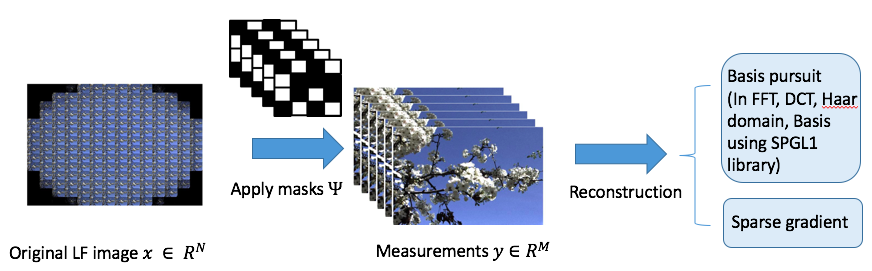
\includegraphics[width=0.95\linewidth, trim={0.3cm 0cm 0.2cm 0.3cm} ,clip]{img/cs_framework.png}
\end{center}
   \caption{The lightfield image reconstruction pipeline. (We take the center $10 \times 10$ angular views from the original lightfield image and resize it by a factor of $6$. Next, we apply random attenuation masks drawn from uniform distribution to get $M$ measurements. Finally, we apply basis pursuit and sparse gradient to reconstruct the lightfield. The original lightfield images were taken from Stanford Lytro lightfield archive. This reconstruction was applied to $24$ images in parallel in Barley.) }
\end{figure}


Reconstructions were performed in parallel for different compression ratios and basis using the Barley machines on the Stanford Farmshare cluster. Each Barley machine is equipped with an AMD Magny Cours (24 cores each) and is shared across multiple users. The approximate time for reconstructing a $90 \times 63 \times 10 \times 10$ lightfield using a particular reconstruction method is shown in Table 1.

\begin{table}
  \begin{center}
  \begin{tabular}{|l|c|}
  \hline
  Basis & Reconstruction Time (hours)\\
  \hline\hline
  Fourier & 12.3 \\
  DCT & 12.4 \\
  Haar & 16.8\\
  TV Prior & 5.1\\ 
  \hline
  \end{tabular}
  \end{center}
  \caption{Reconstruction times for a single lightfield image using the Barley machines.}
\end{table}


We define the SNR as the energy in the original signal divided by the mean squared error of the reconstruction across all colour channels. 

\[SNR = 20 \log_{10}{\frac{||x||_2}{||x_r - x||_2}}\] where $x$ is the original lightfield image, and $x_r$ is the reconstructed lightfield image and $|| \cdot ||_2$ is the $l2$ norm.



\section{Results}

Figure 2 shows the SNR of the reconstructed lightfield images.  From the figure, we see that Haar wavelet basis performs badly when the compression factor is small. The other three methods all reconstruct the image with a high fidelity (average SNR over $20$ dB). In all these four methods, we see the standard deviation of the SNR in images are around $5$ dB which infers the quality of the reconstruction largely replies on the scene. 

Figure 3 shows the reconstructed lightfield images of 3 different images. The top reconstructed image had the lowest SNR of all images chosen, the middle image had the greatest SNR, and bottom had an average SNR among the $24$ images we analyzed. Comparing the characteristics of the three images, we find that reconstruction performs worse in the close-up and non-lambertian scenes than scenes that are lambertian and have a subject that is located further from the camera. This is expected since non-lambertian scenes and scenes where the camera is close to the subject will give more variance when the scene is viewed from a different angle. With respect to compressed sensing, these scenes have less sparsity in the angular domain which makes the assumption on sparsity in angular domain weaker, and the reconstruction less effective. 

Figure 4 further examines the sparsity of the angular domain by comparing the angular images of a poorly reconstructed scene (left image) and a well reconstructed one (right one). Comparing the reconstructions to the original angular images, the scene on the left is not well represented by few coefficients in the DCT or Fourier basis. The reconstruction algorithm approximates the patch as either a single uniform value, or with sinusoids at different frequencies. The reconstruction using the TV prior is best able to capture the variation not captured by comrpessed sensing, which can evidently be seen by looking at the second patch from the right of the left image.

\begin{figure}[t]
\begin{center}
 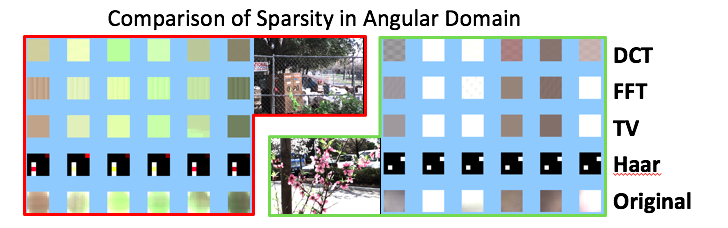
\includegraphics[width=0.95\linewidth, trim={0.0cm 0cm 0cm 0cm} ,clip]{img/patches.png}
\end{center}
   \caption{Comparison of sparsity in angular direction of two images. These lightfield patches are created by taking the same pixel in all of the angular views and assembling them all into one view.
   The original lightfield patch is shown in the bottom row, and the associated reconstructions of that patch in the other rows. This reconstruction is for a compression factor of $0.02$. The left image of a fence is an example of a scene where the angular images are not sparse in the DCT and Fourier basis. This image was reconstructed with an SNR of $13.8$ dB. The right image of a flowering plant is an example of a lightfield where the angular images are sparse in the DCT and Fourier basis. This image was reconstructed with an SNR of $17.2$ dB.}
\end{figure}

\begin{figure}[t]
\begin{center}
 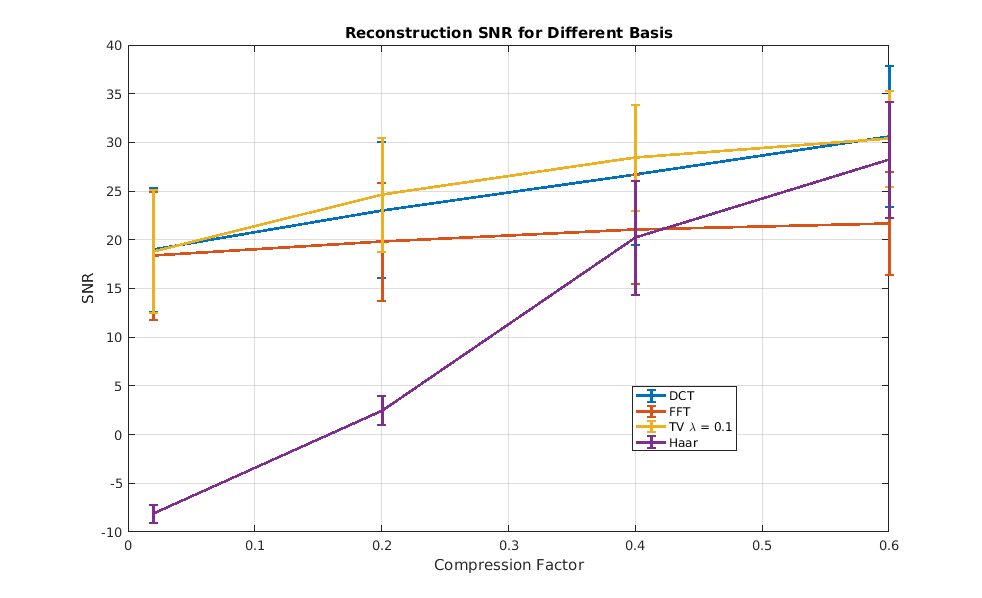
\includegraphics[width=0.95\linewidth, trim={1cm 1cm 1cm 1cm} ,clip]{img/snr_average.png}
\end{center}
   \caption{Reconstruction SNR using TV prior and basis pursuit in DCT, Fourier and Haar Wavelets basis. }
\end{figure}


\begin{figure}[t]
\begin{center}
 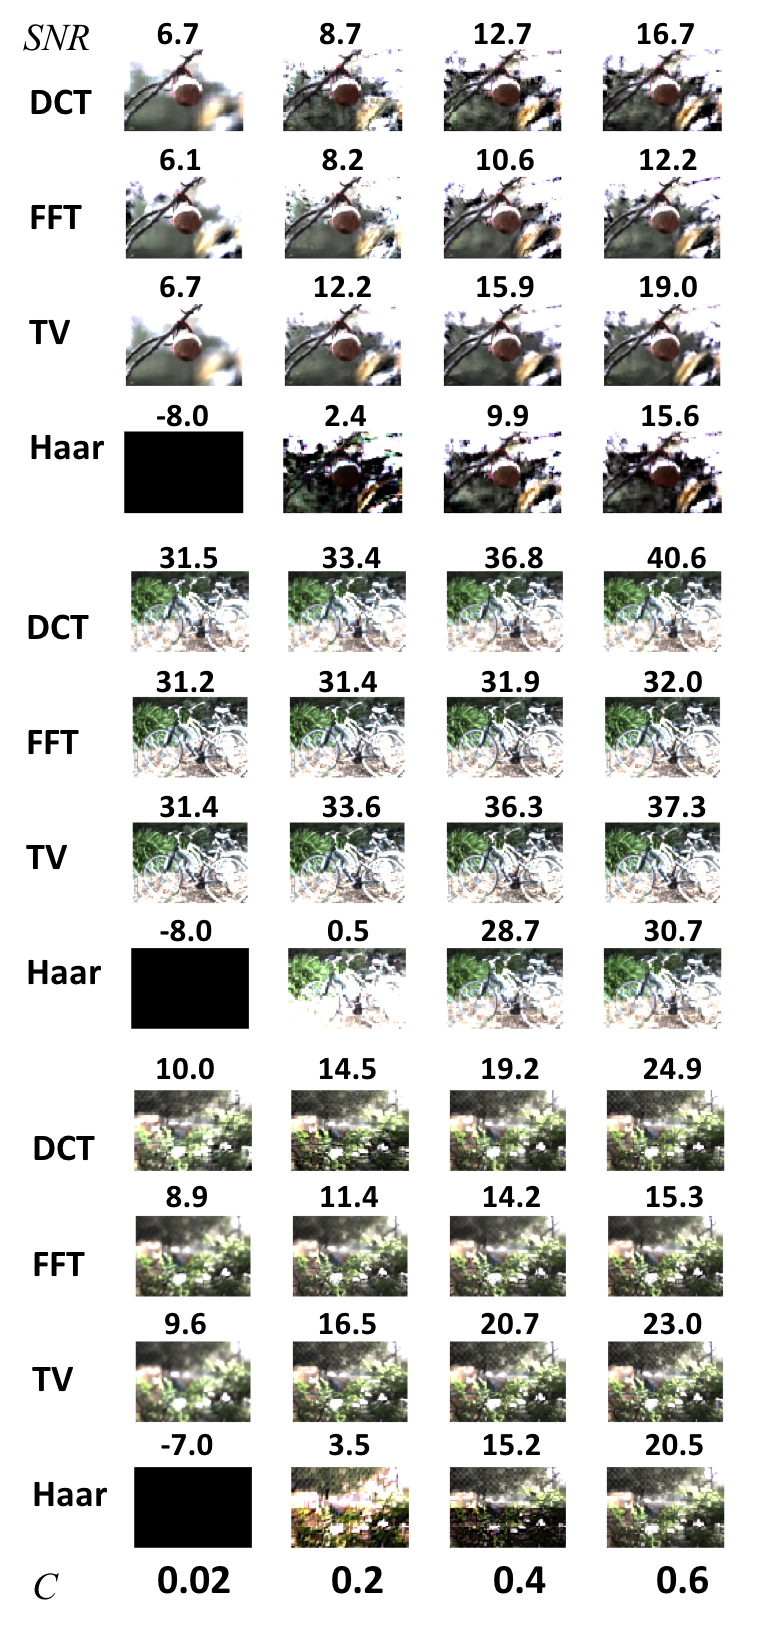
\includegraphics[width=0.95\linewidth]{img/example_images.png}
\end{center}
   \caption{Comparison of reconstruction of three different scenes. From top to bottom are the reconstructed scenes with lowest SNR, highest SNR and a medium SNR. For each scene, we compare the images reconstructed in 4 methods. The SNR value in dB is listed on top of the image. From left to right are the reconstructions at different compression factors.}
\end{figure}

\section{Discussion}


\section{Conclusion}

From the above results, we discovered that sparse gradient method gives us the overall most effective reconstruction in terms of image fidelity and computation time. In contrast, reconstructions using basis pursuit in the Haar wavelet basis performs the worst in terms of both computation time and image fidelity when the compression factor is small. The quality of the reconstruction is also highly dependent on the scene. For scenes where the lightfield is sparse in the angular dimension, the reconstruction works much better than those with little sparsity. This reconstruction can be best applied to scenes lambertian scenes at a distance from our observation. However, the overall computation time required for these reconstructions is prohibitive for consumer applications, and significant progress would have to be made in this regard. 

{\small
\bibliographystyle{ieee}
\bibliography{egbib}
}

\end{document}
